\documentclass[10pt]{article}

\usepackage[a4paper, portrait, margin=0.9in]{geometry}
\setlength{\parskip}{1em}

\usepackage[hidelinks]{hyperref}

\usepackage{graphicx}
\graphicspath{ {./images/} }
\usepackage{caption}
\usepackage{subcaption}
\captionsetup[subfigure]{justification=centering}

\title{Progress Report: Handling Structural Inconsistencies in CT Image Reconstructions}
\author{Cameron Stevenson\\[0.5cm]{\small Supervisor: Ramakrishnan Mukundan}}

\begin{document}
\maketitle

\section{Overview}

This is a progress report for a Computer Science Honours project related to mesh reconstructions from CT image stacks. I will recap the most relevant content of my project proposal and literature survey, and describe my progress in investigating improvements on prior methods. I will also take this opportunity to discuss techniques yet to be investigated and my rationale for them. Finally I will outline my goals and schedule for the remainder of the year.

\section{Introduction}

Medical imaging modalities such as HRCT and MRI produce stacks of images depicting regions of different tissue. These image stacks can be used to reconstruct the 3D structure of internal organs. The renders or models produced are useful in diagnosis, treatment, education, surgical simulation, and robot assisted surgery \cite{mackay2019robust, mukundan2016reconstruction, pan2017comparison}. The process of producing renders or reconstructions can be improved by reducing manual user input, improving reconstruction accuracy, or improving computational efficiency.

Branching structures can be problematic to reconstruct and are a common issue in prior methods. My project aims to improve the accuracy of reconstructions involving branches and other problematic structures. In particular the lungs are used as an organ of focus. 

\section{Background}

Most of my time in this project so far has gone towards a literature survey. I have included the essential details of common methods below, with more elaboration given to the approach relevant to this project. If more detail is necessary refer to my literature survey \footnote{\url{https://github.com/cstevenson3/cosc470writing/blob/main/survey.pdf}}.

\subsection{Generic Methods}

The simplest form of rendering in medical imaging is direct volume rendering \cite{fishman2006volume}. The pixels in the image stacks are treated as voxels, forming a 3D grid of intensity data. Rasterisation or raycasting methods can be applied to these voxels to give a render. These renders are easy to understand and detailed, however they are computationally expensive.

Mesh rendering is preferred for real-time applications, but this requires a mesh reconstruction first. The mesh represents where boundaries of tissue lie in 3D space. To begin with, segmentation of images must be done to find boundaries in 2D space \cite{birkfellner2016applied}. Segmentation methods are usually specific to an organ of interest and are tuned as such. A segmentation gives contours of points representing the boundaries between tissue. These points are then used for mesh reconstructions.

Point cloud methods for mesh reconstruction are adopted from applications like laser scanning, where a lot of points are dumped in as input and the algorithm has to infer which are connected  \cite{oztireli2009feature}. The contour points from segmentation can be used as input in a point cloud method to produce a reconstruction. Point cloud methods typically interpolate from points and don't use them directly in the output mesh.

Marching cubes is another method for mesh reconstruction \cite{lorensen1987marching}. Boundary voxels are found, and their neighbouring voxels are considered in a lookup table to decide what local triangulation should be made for that voxel. All the triangles are then connected for the whole mesh. Marching cubes produces jagged results and ambiguity can lead to defects.

\subsection{Correspondence Methods}

A more direct approach to mesh reconstruction is to decide which contours should be connected, then triangulate between them, with an optional point correspondence step in the middle. Such an approach produces output meshes which contain the original points. The result is a method which gives computationally faster renders than direct volume rendering, potentially more accurate meshes than point cloud methods, and a smoother mesh than marching cubes. Mackay \cite{mackay2019robust} presents one such paper to use this approach, and my project focusses on extending his method.

\subsubsection{Contour Correspondence}

Contour correspondence takes as input all the contours in a segmentation of an image stack, and produces as output matchings of contours which should be connected. In a simple case a matching would be one contour in one slice and a similarly positioned contour in an adjacent slice. In more complicated cases such as branching there may be one-to-two matchings. Metrics for matching include centroid position closeness, size and shape similarity etc.

Correspondence algorithms can operate on different levels:
\begin{itemize}
\item local: looking only at adjacent slices each iteration
\item global: looking for the best matching across all slices each iteration
\item growing: keeping a hierarchy of connected components, and adding unmatched contours onto these components each iteration
\end{itemize}

\subsubsection{Point Correspondence and Triangulation}

With contour correspondences established, points in matched contours must themselves be matched to create a triangulation for a mesh. Points can be matched by Euclidean distance, and by their index within a contour. 

Mackay \cite{mackay2019robust} proposes Dynamic Time Warping (DTW) as a method of point correspondence. DTW matches features on the same structure which has been slightly warped, making it suitable for contours on adjacent slices which should differ only slightly. DTW generates a warping path going around both contours, producing point matches as it goes. Euclidean distance is used as the cost function, and some constraints are put on the warping path to keep it progressing on both contours in case Euclidean distance is not suitable for a section.

Triangulation is relatively simple, taking point correspondences as edges and filling gaps where necessary. Ideally the two contours have similar sizes otherwise many triangle fans will be created, which gives a rougher mesh.

\subsubsection{Branching Problem}

Branching structures are problematic to reconstruct. When scanned they show up as one contour in one slice and two contours in the next slice. There is ambiguity in contour correspondence, as this could represent many possible structures (a branch, a bend, the end of one tube near another tube). Mackay \cite{robust2019construction} looks for lung branches as one contour approximately splitting in half into two nearby contours.

When it comes to point correspondence, branches affect the position of points drastically and so correspondence metrics are skewed. In Mackay's \cite{mackay2019robust} method DTW requires two ordered contours as input, so the two-contour side of the branch must be merged into a single contour first. DTW does not handle all branching cases well, with some twisting and too many points matched to a single point. Fixing this is left as further research.

\section{Progress}

Following the literature survey, I found a week to begin trialling new techniques to improve correspondence methods, with the intent of handling branching structures better. I am using Mackay's method and C++ code as a base to work from, adding modifications as I go. Fortunately Mackay's code is well structured and easy to drop in modifications to test. I took one day to set up my environment and run the original code successfully. I then took four days to try my first idea in python, port it over to C++, and substitute it into Mackay's code.

\subsection{Point Angle Rationale}

The first idea I tried began with me observing twisting produced by DTW in branching cases. I hypothesised two reasons for this. Firstly the choice of starting point in each contour was the leftmost point (lowest x value). For similarly shaped contours this should give roughly the same point in each contour (in an intuitive sense). However in branching cases where the two-contour merged contour is oriented mostly in the z-direction, the leftmost point could be either on the top or bottom contour, whereas on the single contour it would be towards the middle. A great difference in starting point location would cause triangle fanning at the start and end of DTW. Secondly, a scanned structure progressing at an angle through the scan planes would have contours shifted away from each other. Since DTW relies on Euclidean distance as a cost function, I hypothesise this shift would bias which points are matched, ignoring the underlying structure.

For the above two reasons my first trialled idea was to calculate the centroids of matched contours, and translate them to the origin for point correspondence. This allows for choosing of a starting point near the x-axis (the rightmost point), and so starting points are better aligned between contours. With this translation made, it opened up the opportunity to try an alternative pathing algorithm. My idea was to use point angle from the now shared centroid to match points across contours. In ideal conditions each contour would have one point per angle, but this is not the case, particularly in merged contours. For the pathing algorithm I required monotonicity, so for each point if a prior point on the ordered contour had a greater angle I used this as the angle for the current point. This produces segments of points with the same angle, and so I added in a second metric to keep the path moving. This metric was progression along the contour, measured simply as how many points had been passed out of the total number of points. A weighted sum of the angle and progression metrics is used in the pathing algorithm. A current pair of points is kept, and points on each contour are leapfrogged between such that whichever point is behind on a metric is advanced to the next point. All pairs are recorded to give the point correspondence. I refer to this method as point-angle.

\subsection{Point Angle Testing}

Mackay provides the synthetic models used for testing his method, with contours sampled on planes cut through the model. I used the "multi-branch" model sampled with 10 and 50 planes, focussing on the middle branch and the lower branch. I ran the reconstruction with DTW and with my point angle method at various weightings for the angle of points vs. the progression of points. Although quantitative accuracy testing is possible (and will be done in future), with the limited time I had I elected to begin with a visual comparison to screen my method for viability. 

\begin{figure}[h]
     \centering
     \begin{subfigure}[b]{0.22\textwidth}
         \centering
         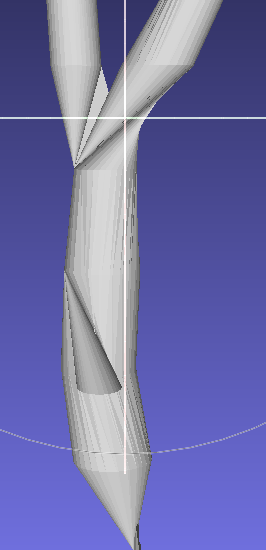
\includegraphics[width=\textwidth]{dtw10}
         \caption{DTW \linebreak}
         \label{fig:dtw10}
     \end{subfigure}
     \hfill
     \begin{subfigure}[b]{0.2\textwidth}
         \centering
         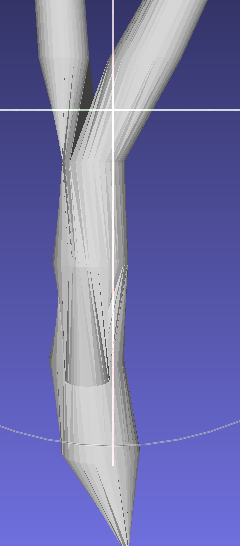
\includegraphics[width=\textwidth]{pa10ang00}
         \caption{Point angle, 0\% angle weight}
         \label{fig:pa10ang00}
     \end{subfigure}
     \hfill
     \begin{subfigure}[b]{0.195\textwidth}
         \centering
         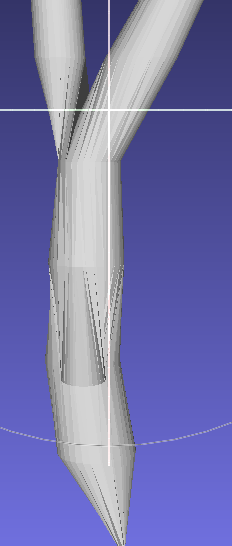
\includegraphics[width=\textwidth]{pa10ang50}
         \caption{Point angle, 50\% angle weight}
         \label{fig:pa10ang50}
     \end{subfigure}
     \hfill
     \begin{subfigure}[b]{0.2\textwidth}
         \centering
         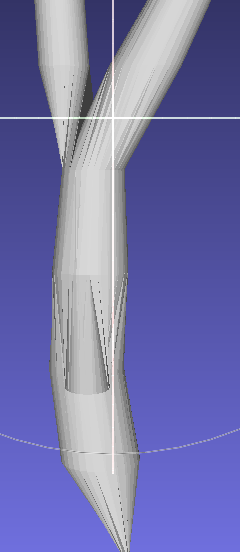
\includegraphics[width=\textwidth]{pa10ang100}
         \caption{Point angle, 100\% angle weight}
         \label{fig:pa10ang100}
     \end{subfigure}
        \caption{Reconstructions with 10 plane samples}
        \label{fig:plane10}
\end{figure}

\begin{figure}[h]
     \centering
     \begin{subfigure}[b]{0.215\textwidth}
         \centering
         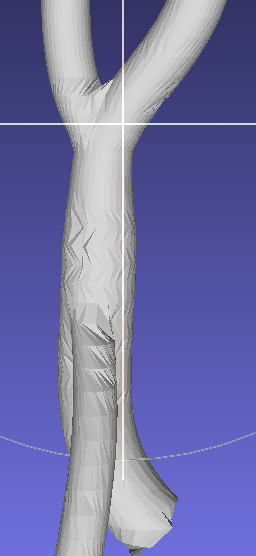
\includegraphics[width=\textwidth]{dtw50}
         \caption{DTW \linebreak}
         \label{fig:dtw50}
     \end{subfigure}
     \hfill
     \begin{subfigure}[b]{0.2\textwidth}
         \centering
         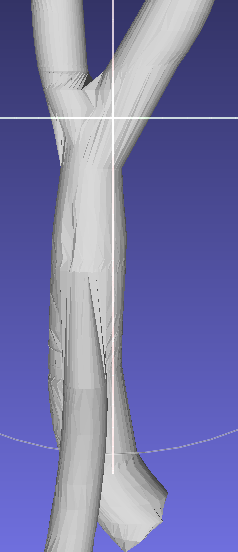
\includegraphics[width=\textwidth]{pa50ang00}
         \caption{Point angle, 0\% angle weight}
         \label{fig:pa50ang00}
     \end{subfigure}
     \hfill
     \begin{subfigure}[b]{0.205\textwidth}
         \centering
         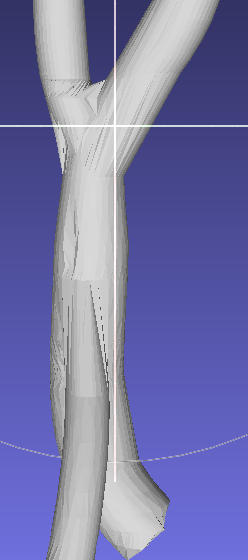
\includegraphics[width=\textwidth]{pa50ang50}
         \caption{Point angle, 50\% angle weight}
         \label{fig:pa50ang50}
     \end{subfigure}
     \hfill
     \begin{subfigure}[b]{0.2\textwidth}
         \centering
         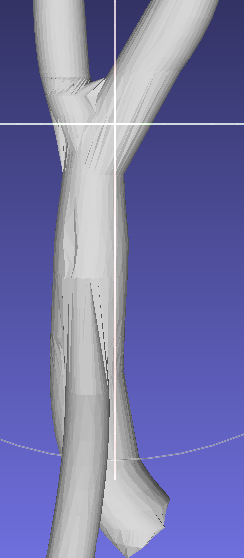
\includegraphics[width=\textwidth]{pa50ang90}
         \caption{Point angle, 90\% angle weight}
         \label{fig:pa50ang90}
     \end{subfigure}
        \caption{Reconstructions with 50 plane samples}
        \label{fig:plane50}
\end{figure}

Observations:
\begin{itemize}
\item At lower plane sampling rates, my point angle method gives better results than DTW in the simpler tube sections and in the branching sections. The lower tube now originates from a region rather than a single point, and the middle branch now has no twisting. However the middle branch left side still originates from a point, so point angle has not improved on DTW in this regard.
\item Angle weighting has a low impact on correspondence in branching structures. Higher angle weightings produce smoother triangulations in the simpler tube sections, most noticeable in the low plane sampling rate. At higher plane sampling rates DTW has this "wavy" effect as twisting direction jumps back and forth, presumably because of the choices of starting points in contour pairs. In point angle there is no noticeable twisting, which is an improvement on DTW.
\item At higher plane sample rates, DTW has a cleaner overall structure. Point angle has some extraneous triangulation near bends.
\end{itemize}

Thoughts:
\begin{itemize}
\item DTW and point angle each have strengths and weaknesses depending on plane sampling rate, and what type of contour correspondence is being acted on. The program is aware of these factors, and so could switch between the two methods for each contour match depending on the circumstance. For example at high plane sampling rates DTW could be used to get cleaner branches, whilst point angle is used for the simpler tube sections to give smoother results.
\item Point angle method is limited by the fact that merged contours in branching structures do not have one point per angle.
\end{itemize}

\section{Future}

\subsection{Schedule}

I have a 3 week mid year break in which to trial further improvements, and this momentum should continue into term 3. As I go along I will familiarise myself with the quantitative testing used by Mackay. My aim is to have found a significant improvement by mid August, giving me something valid to present at the CSSE Postgraduate Conference in early September. After the conference I will have 7 weeks to test my proposed solution against Mackay's and write up my final report. With the literature survey already complete, and Mackay's mesh testing methods to refer to when needed, there should be no major setbacks in producing this report. Overall I am confident I am on schedule to find an improvement and meet the Honours course deadlines.

\subsection{Potential Improvements}

\subsubsection{Contour Correspondence}

\subsubsection{Point Correspondence}

Before the point angle method I translate contours so their centroids align. I want to try also rotating contours so that their major axes align. I will do this because I noticed that branch reconstructions under DTW tend to be lower quality when the branch is oriented in the z-direction. Aligning contours by rotation will help with selecting good starting points, and ensure that real twisting of structures is inferred in the reconstructions. I then want to take these transformations and apply them before DTW, as I believe it will improve the way DTW behaves.

Mackay merged contours in branching cases on the two-contour side. I want to try splitting the contour on the one-contour side instead. I believe this will make for cleaner branch triangulations.

\pagebreak
\bibliographystyle{IEEEtran}
\bibliography{references}

\end{document}
